\chapter{Introduction}
\label{cpt:intro}
The appearance of a scene can often provide an abundance of information about the scene including time of day, location, and weather. With all of this information available, it is up to us to find ways to automatically extract it from images of the scene to allow a better understanding of what is going on at a given location. This thesis will attempt to use the information collected by webcams to infer information about environmental signals such as wind velocity and vapor pressure. 

One of the primary challenges of predicting weather signals from images is that the images may vary more due to other causes such as time of day than those which relate to our signals of interest. Thus, we begin by exploring mechanisms for learning features that are invariant to other scene changes. Through the use of correlation techniques such as Canonical Correlation Analysis (CCA), we find that we are able to extract useful information from webcam images which allow us to predict local weather data. This will help us gain a better understanding of local weather patterns and variations as well as fill in missing weather data entries, which occur quite frequently. Furthermore, this allows us to use the abundantly existing webcams all over the country as crude weather sensors, to complement the government weather stations spread out sparsely across the country. 

This thesis will go through the background information, motivation, and related work in Section \ref{cpt:intro}. It will then discuss the theory and details of the correlation techniques used in Section \ref{cpt:cca}. Section \ref{cpt:results} will begin to show the application and results of the aforementioned methods. It will also show experiments to determine the appropriate size of the training set necessary to avoid any biases in the images or over training of the predictors. We will conclude  and propose future work on this problem in Section \ref{cpt:conclusion}.

\section{Related Work}
This thesis build on existing work in collecting large image datasets and the use of correlation analysis tools, specifically CCA.

Working with large webcam datasets represent many challenges and provide many opportunities for interesting research. Recent work has been seen in understanding all the variations in a given scene over time using a single statically controlled camera \cite{CAVE_0059}. This knowledge of the possible variations such as illumination and weather make it possible to de-fog, de-haze, and generally improve the quality of images captured in bad weather conditions. Larger, more uncontrolled datasets have been used to test geolocation \cite{jacobs07geolocate} and orientation \cite{jacobs08geoorient} algorithms. Additionally, webcam dataset have been used to infer geographic location from single images \cite{im2gps} by estimating the distribution across the entire world, and to determine camera calibration variables by using the sky appearance and sun position \cite{lalonde-eccv-08}.

CCA is a regression technique \cite{hotelling} which has been used frequently in statistical analysis through the years. It has recently been used as a means to correlating sounds with frames in movies to develop a system to recall movie scenes based on the associated sounds \cite{957143} such as explosions, or crying. It has also been used, with success, as a key algorithm in content-based image retrieval systems \cite{1119703}. The work presented here will look to take CCA and apply it to a large, diverse set of webcams to infer information about the weather.

\section{Background Information \& Dataset}
The Archive of Many Outdoor Scenes (AMOS) database \cite{jacobs07amos} has been collecting images from 835 webcams every 30 minutes since March 2006 and now contains over 40 million images. The AMOS dataset is unique in providing time-stamped images from many cameras around the world. No other dataset provides the broad range of geographic locations and the long temporal duration that is does. This database is the largest known collection of natural scenes collected from static cameras and as such offers a wealth of data to test our methods against. While there are cameras located across the world, we focus on those located within the continental United States so that ground truth weather data can be collected.

The weather data is collected from the Historical Weather Data Archives (HWDA) \cite{noaa} which is maintained by the National Oceanic and Atmospheric Administration (NOAA). The archives maintain a large variety of weather data from January 1, 1933 through present day collected hourly on just over 6,000 weather stations located across the continental United States. The data collected includes, but is not limited to, wind velocity, precipitation, temperature, relative humidity, vapor pressure, cloud conditions, dew points, and various aggregated data signals.

\chapter{Canonical Correlation Analysis (CCA)}
\label{cpt:cca}
The main correlation technique which we will explore is a method called Canonical Correlation Analysis (CCA) \cite{hotelling}. The goal of CCA is to find two transformation matrices $A$ and $B$ to maximize the correlation between two independent data sets $X \in \mathbf{R}^{x\times n}$ and $Y \in \mathbf{R}^{y\times n}$. In other words, CCA looks to find $A$ and $B$ such that $AX\approx BY$. CCA is a way of finding a linear relationship between two independent, multidimensional variables.

The matrices $A$ and $B$ are build column by column. At each step, CCA seeks to find vectors $a$ and $b$, called canonical variables, to maximize the correlation:
\begin{equation}\label{eq:maxcorrcca}\rho = corr(aX,bY),\end{equation}
while minimizing the correlation of $a$ and $b$ with all of the canonical variables already found. The vectors are then added to $A$ and $B$ respectively as new rows. This is continued $min(x,y)$ times where $x$ and $y$ are the lengths of the two datasets.

What makes CCA different from other correlation methods is its invariance to affine transformations of the input variables. In other words, CCA will be able to find a linear relationship between two multidimensional variables even if different coordinate systems are used for each variable \cite{bkl97}. This makes CCA a very desirable method for relating image data to environmental signals, which are clearly not measured in the same coordinate system. One very crucial component of CCA is that while the input matrices $X$ and $Y$ can have a varying number of dimensions, they must have \textit{exactly} the same number of samples in order to find a CCA relationship between two multi-variable signals. Because our sensors samples on their own schedules, this requires us to remove some entries in order to have the same number of samples in each dataset.

\section{Applications}
We will now focus on the application of CCA to predicting time-varying weather signals from image sequences over the same time period. Given the localized nature of weather data, we assume that the weather station used for ground truth weather data is located near to the camera in order to maximize the accuracy of our predictions. The algorithm takes as input a set of images $I=i_1\ldots i_a$ and a set of weather observations $W=w_1\ldots w_b$. The method will assume the availability of images and weather data with corresponding timestamps. In order to ensure that this invariant holds, the first step of the algorithm is to run through both datasets and remove entries that do not have a corresponding entry in the other dataset. This is done by concurrently iterating through both sets and finding entries with matching timestamps within some given threshold $\epsilon$. Entries without a matching component in the other set are removed. This step guarantees that all of the data samples match and that there are an equal number in both sets, which is required for CCA. Now, the input is of the form $I=i_1\ldots i_n$ and $W=w_1\ldots w_n$.

\begin{figure}
	\centering
		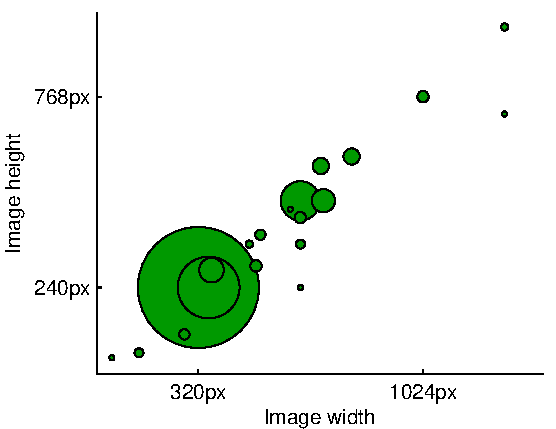
\includegraphics{figures/imagedimensions.pdf}
	\caption[The distribution of image sizes in AMOS, measured in pixels]{The distribution of image sizes in AMOS, measured in pixels. The circles are centered at the width and height of the image and their sizes are proportional to the number of webcams which output images of that size in the AMOS dataset.}
	\label{fig:imagedimensions}
\end{figure}

Once the datasets are properly aligned, we turn our attention to the images. Figure \ref{fig:imagedimensions} shows us that the most common size image from a webcam in the AMOS dataset is $320\times 240$ pixels, which means one image can be expressed as a $1\times 76800$ vector. This is clearly a very costly and inefficient way to store image data, especially when CCA will require a few hundred images to build a good predictor. In order to reduce the storage size for each image, and as a result accelerate the runtime of our algorithms, Principal Component Analysis (PCA) will be applied to the images as a way to find the $k$ most important features from the images and then express each image as a linear combination of these features ($k$=10 is used here). 

PCA will take as input a set of images $I$ and will return three matrices $U\in \mathbf{R}^{m\times k}$, $S\in \mathbf{R}^{k\times k}$, and $V\in \mathbf{R}^{k\times n}$ where $m$ is the length of a single image when expressed as a vector. $U$ contains the $k$ orthogonal feature vectors, $S$ is a diagonal matrix where the elements represent the relative importance of each of the $k$ features, and $V$ contains the coefficients of each of the $k$ feature vectors for each of the $n$ images ($v_i$ contains the coefficients for the $i$th image). We can thus create reconstructions of the images by multiplying $U$, $S$, and $V$ back together. In mathematical terms, PCA attempts to find $U$, which is made up of $k$ orthogonal feature vectors such that we minimize:
\begin{equation}\sum_{i=1}^{n}{\left(I_i - USv_i\right)^2}\label{eq:pca}\end{equation}
PCA will extract significant scene variations from the set of input images which, when used to reconstruct the original images, will minimize the reconstruction error. We now have a way to express each image as a $1\times k$ vector, which is significantly smaller than the original image and contains the most important variations. This will be part of the input into CCA.

The PCA coefficients for each image stored in $V$ and the corresponding weather data $W \in \mathbf{R}^{y\times n}$ will be the input matrices for CCA. After running CCA, we will have projection matrices $A$ and $B$. These can now be used to predict weather data from new images which were not included in the input for CCA. Given a new image $i$, we begin by obtaining the $k$ PCA coefficients by projecting the image onto our existing basis vectors stored in $U$. We can now take those coefficients in a vector $\mathbf{v}$ and use them to predict the associated weather values $\mathbf{w}$ as follows:
\begin{equation}\label{eq:predict}\mathbf{w}=A\mathbf{v}B^{-1}\end{equation}
This is the key equation that is used to extract the inherent weather data from an image. The next section applies these algorithms to actual data sets and present some results as well as additional information which can be extracted, including the minimum size of the training set and the orientation of the camera.

\chapter{Results \& Analysis}
\label{cpt:results}
Two weather signals are considered as driving examples: wind velocity and vapor pressure. These two signals present unique challenges and opportunities. The effect of wind velocity is limited to locations in the scene that are affected by wind, such as flags and vegetation. On the other hand, vapor pressure may affect the scene in a more broad and subtle manner. Choosing two examples with such unique characteristics is a way to test whether the algorithm is able to handle a variety of weather signals or if it is best suited for certain classes of measurements.

\section{Wind Velocity}
Wind velocity is a signal whose effects are only seen in certain local parts of the image; objects such as building and cars will be unaffected by changes in wind. In order to ensure that wind can be accurately predicted, a camera is chosen which contains a flag (Figure \ref{fig:windspeedextremes}). 
\begin{figure}
	\centering
		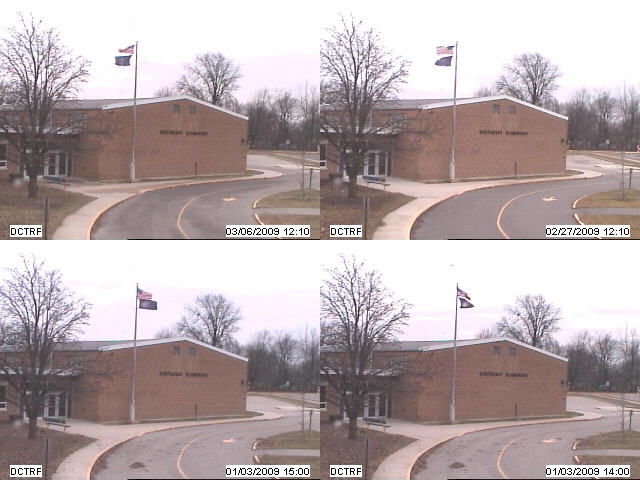
\includegraphics[width=0.60\textwidth]{figures/windspeedextremes.jpg}
	\caption[Some sample images from camera $\#$194 of the AMOS database located in Decatur, IN]{Some sample images from camera $\#$194 of the AMOS database located in Decatur, IN. The presence of a flag on top of the school building is key to the ability to predict wind velocity.}
	\label{fig:windspeedextremes}
\end{figure}

The CCA projections are trained on 204 images collected between January 1 and February 11, 2009. In order to focus on variations in the scene due to weather, we only use images captured between 10 AM and 2 PM local time. Doing this can successfully remove most of the variation caused by time of day and the resulting shadows. The wind velocity is made up of a wind speed in meters/second and a direction in degrees, which we convert to north/south and east/west components using basic trigonometry, and was collected from the closest weather station to the camera. 

Based on this data, we would expect the two dimensions of the CCA projection matrix $A$ to predict the north/south and east/west components of the wind speed. After running CCA, the matrix $A$ is projected onto the feature vectors $U$ from the PCA analysis of the images in order to visualize the canonical features extracted by CCA. As we see in Figure \ref{fig:windspeedcomponents1}, CCA clearly identifies the position of the flag as the crucial indicator of wind speed. Furthermore, we can also notice slight variations in the tree positions, which also are affected by wind speed. The projection of the second basis vector, which can be seen in Figure \ref{fig:windspeedcomponents2} is far less accurate and does not yield an accurate prediction of the other component of the wind speed. This indicates that wind velocity can only be accurately predicted along one of the two components. While this is not a favorable result, it is plausible and agrees with our assumptions; the flag captured in a 2D image can clearly only predict wind speed along one vector. The hypothesis that only the first CCA component is useful is further verified with the correlation values of the predicted values from each component with the actual values $(r_1=0.61759, r_2=0.3523)$
\begin{figure}
	\centering
	\subfigure[]{
		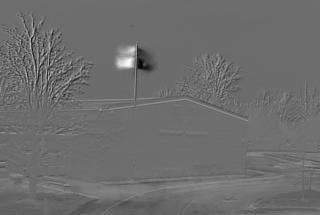
\includegraphics[width=0.45\textwidth]{figures/windspeedcomponents1.jpg}
	\label{fig:windspeedcomponents1}
	}
	\subfigure[]{
		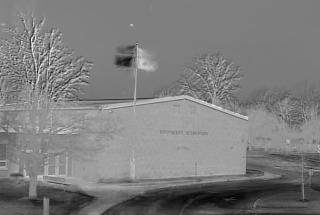
\includegraphics[width=0.45\textwidth]{figures/windspeedcomponents2.jpg}
	\label{fig:windspeedcomponents2}
	}
		\caption[CCA basis vectors for wind velocity projected onto the image space]{Figure \ref{fig:windspeedcomponents1} shows the projection of the first basis vector from CCA onto the original image space. It is clear to see that the position of the flag and the trees are the major variations. Figure \ref{fig:windspeedcomponents2} shows the projection of the second basis vector and is far less accurate than the first.}
\end{figure}

We can now use equation \ref{eq:predict} to infer the magnitude of the wind velocity on 102 images collected between February 11 and March 17, 2009 which were not used in the training of the CCA. Figure \ref{fig:windpred} shows a plot of the ground truth values for wind speed as well as the predicted values using CCA. The associated images below the plot correspond to the filled markers and clearly indicate that the wind speed predictions not only agree with the ground truth values but also directly correlate with the direction of the flag. These results, along with the scatter plot in Figure \ref{fig:windspeedcorr} strongly support our belief that wind speed along a given vector can be predicted based on the position of the flag.
\begin{figure}
	\centering
	\subfigure[]{
		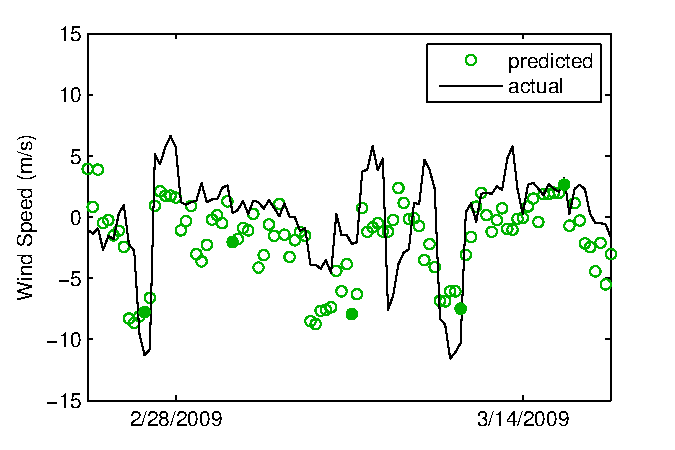
\includegraphics[width=0.60\textwidth]{figures/windspeedtimeseries.pdf}
		\label{fig:windspeedtimeseries}
	}
	\subfigure[]{
		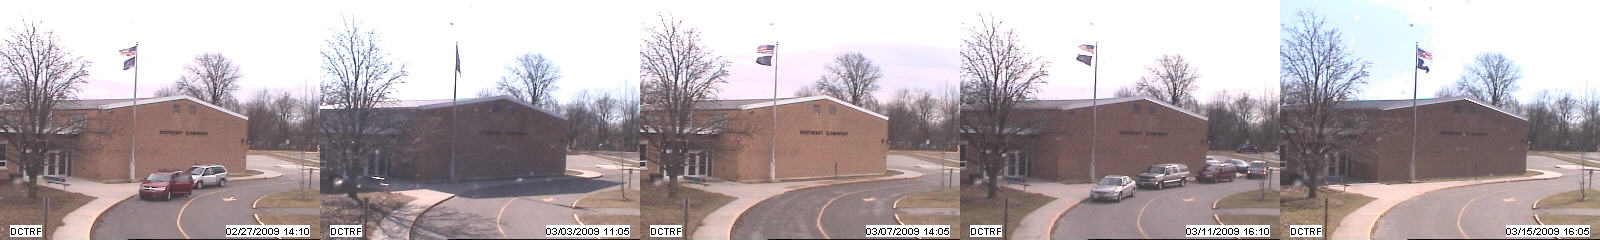
\includegraphics[width=0.90\textwidth]{figures/windspeedtimeseriesimages.jpg}
		\label{fig:windspeedtimeseriesimages}
	}
	\caption[Predicted wind speed values and corresponding ground truth values in meters/seconds]{Predicted wind speed values and corresponding ground truth values in meters/seconds shown in Figure \ref{fig:windspeedtimeseries}. Each image in Figure \ref{fig:windspeedtimeseriesimages} is associated with one of the filled markers in the plot above.}
	\label{fig:windpred}
\end{figure}
\begin{figure}
	\centering
		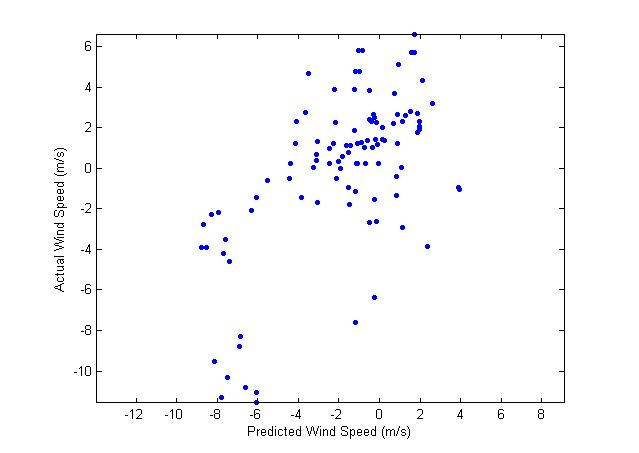
\includegraphics[width=0.60\textwidth]{figures/windspeedcorr.jpg}
	\caption[Scatter plot of predicted wind speed values vs. actual wind speed values]{Scatter plot of predicted wind speed values vs. actual wind speed values. $(r=0.61759)$}
	\label{fig:windspeedcorr}
\end{figure}

Although we are unable to predict both components of the wind speed, there is still some more information can be extracted from the results. Namely, we can use the known actual wind directions with our predicted wind speed along some unknown vector to solve for the direction of that vector. This vector will allow us to determine the orientation of the camera in the world.

We will find this vector by solving a simple matrix equation of the form $Ax=b$. $A \in \mathbf{R}^{n\times 2}$ are the known wind speeds in north/south and east/west components and $b \in \mathbf{R}^{n \times 1}$ are the predicted wind magnitudes. Thus, solving for $x$ will yield the orientation of our camera in the world, which is also the vector along which we observe the flag blowing. Figure \ref{fig:winddirpred} shows a scatter plot which visualizes the relationship between the actual wind vectors and predicted wind magnitudes, along with the vector $x$ solved for using the above equation. The same line is also shown overlaid onto an actual satellite image of the known camera location. We see that this vector clearly 
\begin{figure}
	\centering
	\subfigure[]{
		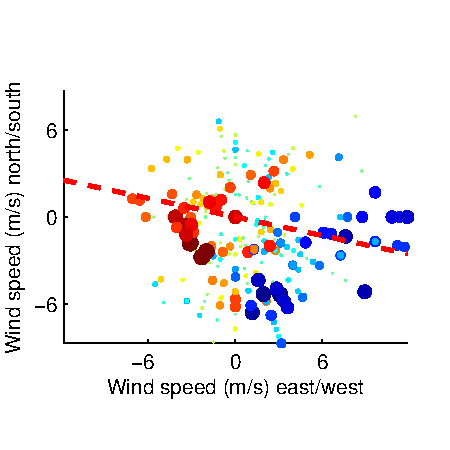
\includegraphics[width=0.45\textwidth]{figures/windspeedscatter.pdf}
		\label{fig:windspeedscatter}
	}
	\subfigure[]{
		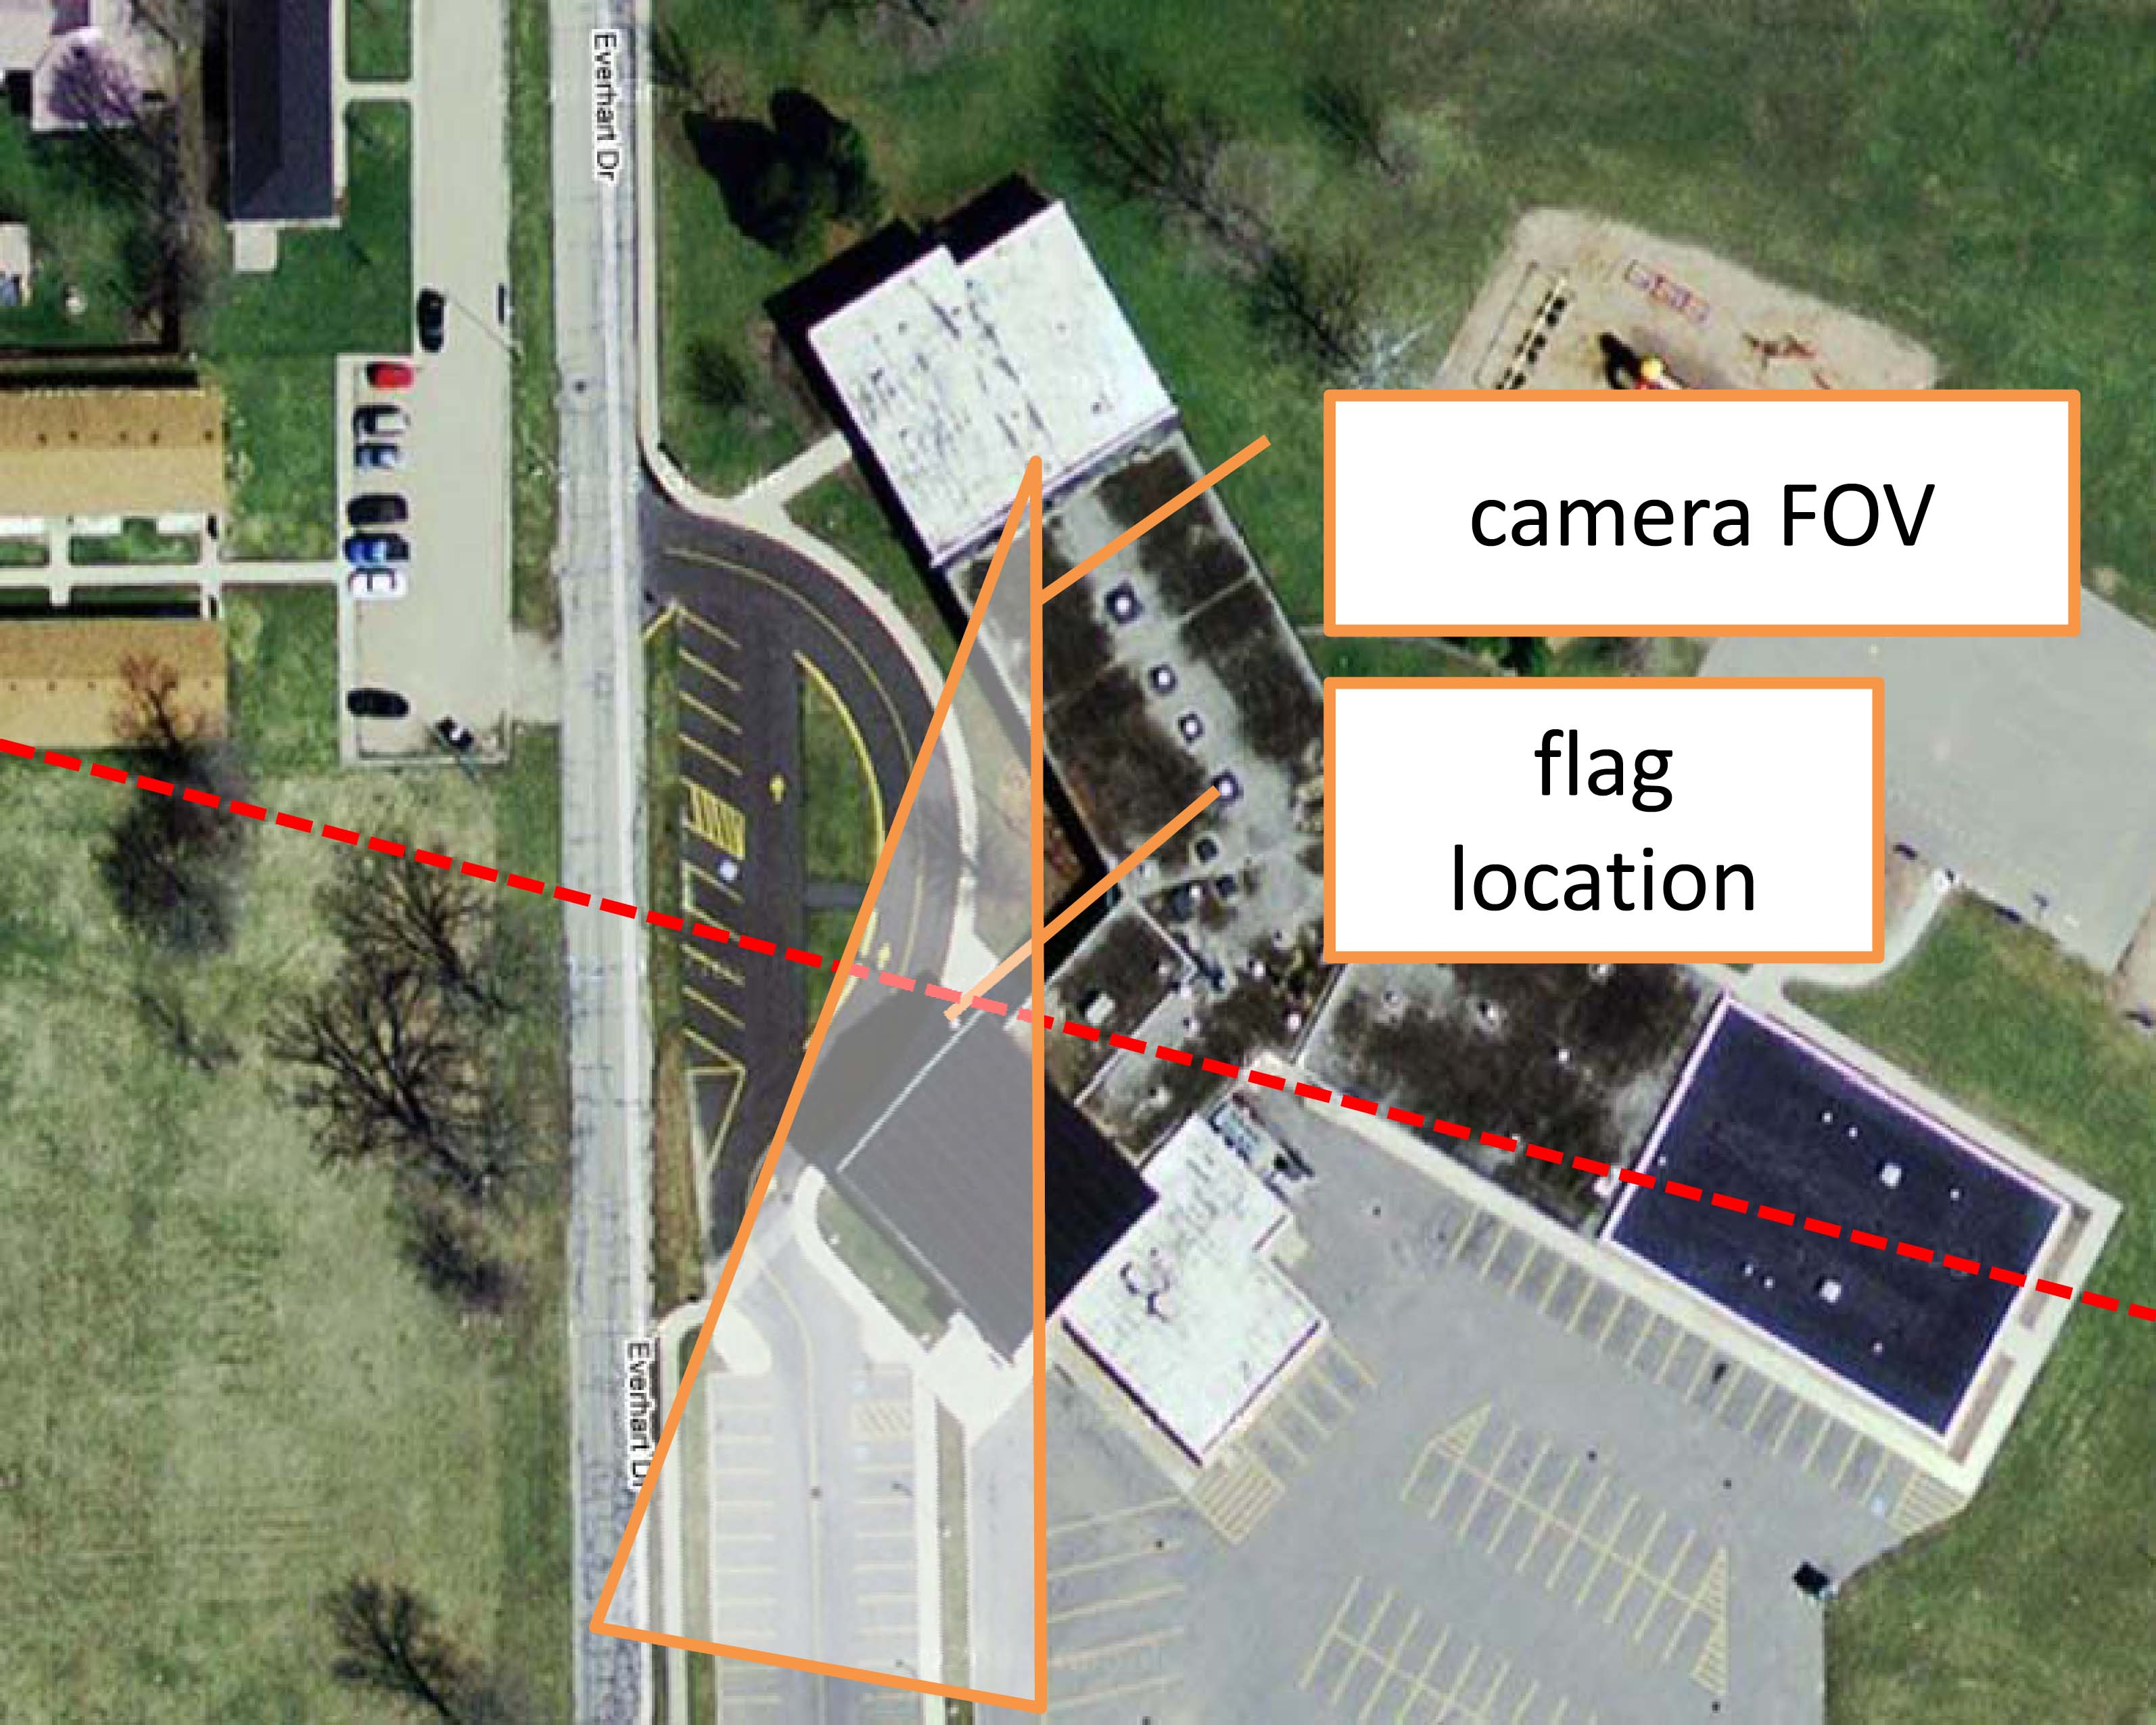
\includegraphics[width=0.45\textwidth]{figures/decaturin.jpg}
		\label{fig:decaturin}
	}
	\caption[Further analysis of the wind speed predictions provides a way to predict the axis along which the flag is blowing]{Further analysis of the wind speed predictions provides a way to predict the axis along which the flag is blowing. In Figure \ref{fig:windspeedscatter} the size and color of each marker is determined by the predicted wind speed and the location of each marker is determined by the north/south and east/west components of the actual wind speed at the same time. The dashed red line is the normal to the projection axis determined by running linear regression between the predict and actual values. Figure \ref{fig:decaturin} shows this axis overlaid on a Google Maps image with the field of view crudely estimated by hand. We see that the predicted vector is nearly parallel to the field of view, which means that it indicates the orientation of the camera correctly.}
	\label{fig:winddirpred}
\end{figure}

\section{Vapor Pressure}
The second example will consider the weather signal of vapor pressure, which is the contribution of water vapor to the overall atmospheric pressure and is measured in millibars. Since this is a 1-dimensional signal, unlike wind velocity, running CCA is essentially equivalent to linear regression. A camera is chosen which contains a distant skyline of buildings as well as a view of the sky and horizon (Figure \ref{fig:vaporextremes}). The hypothesis is that as vapor pressure increases, the overall clarity of the distant skyline will decrease due to haze and clouds. The primary challenge with vapor pressure as opposed to wind speed is that it is a signal which effects the entire scene as opposed to a localized area, and is not quite as easy to comprehend visually.

The CCA projections for this example were trained on 198 images captured from January 1 to February 19, 2009. Once again, we only consider images between 10 AM and 2 PM as a way to ignore variations due to time of day.
\begin{figure}
	\centering
		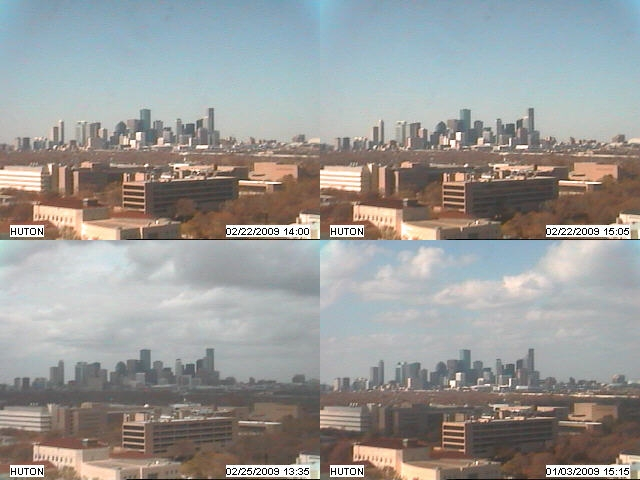
\includegraphics[width=0.60\textwidth]{figures/vaporextremes.jpg}
	\caption[Some sample images from camera $\#$619 of the AMOS database located in Houston, TX]{Some sample images from camera $\#$619 of the AMOS database located in Houston, TX. The visibility of the distant skyline of buildings as well as the presence of clouds to helps to predict vapor pressure.}
	\label{fig:vaporextremes}
\end{figure}

Unfortunately, when the algorithm is run exactly as described above, we get poor results that do not correlate very strongly with what we expect to change with vapor pressure. As is seen in Figure \ref{fig:vaporcomponents1-nongrad}, the reprojection of the single dimension of CCA does not yield a very convincing image. It appears that the CCA projection has identified the position of the sun against the buildings as one of the important factors, which may not always correlate with vapor pressure. Since CCA identified this seemingly unrelated signal, the predictions yield a mediocre correlation $(r=0.3894)$ between themselves and the actual values, as seen in Figure \ref{fig:vaporcorrb}. In order to improve the predictions and identify a relevant feature in the image, the original images are replaced with their gradient magnitude images, which are computed as follows:
\begin{equation}\label{eq:grad}I_g=\sqrt{\frac{dI}{dx}^2 + \frac{dI}{dy}^2}\end{equation}
The gradient images will tend to highlight edges and other major changes in the images. The projection of the CCA basis found when using these gradient images can is in Figure \ref{fig:vaporcomponents1} and, as we can see, clearly focuses on the visibility of the edges of the buildings, which is what was hypothesized to change with vapor pressure. Additionally, we get a stronger correlation between the actual and predicted values when using the gradient image $(r=0.73684)$.
\begin{figure}
	\centering
	\subfigure[]{
		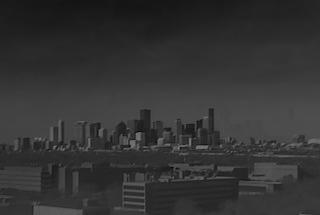
\includegraphics[width=0.45\textwidth]{figures/vaporcomponents1-nongrad.jpg}
		\label{fig:vaporcomponents1-nongrad}
	}
	\subfigure[]{
		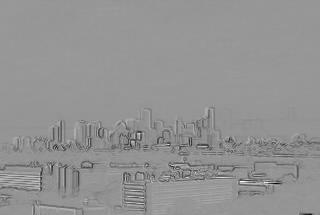
\includegraphics[width=0.45\textwidth]{figures/vaporcomponents1.jpg}
		\label{fig:vaporcomponents1}
	}
	\caption[The projections of the CCA basis vector computed with the regular and gradient images]{The projections of the CCA basis vector computed with the regular and gradient images, respectively. Figure \ref{fig:vaporcomponents1-nongrad} does not identify a feature which actually correlates strongly with vapor pressure. However, when using the gradient image instead in Figure \ref{fig:vaporcomponents1}, the CCA basis clearly identifies the visibility of the skyline as an indicator of vapor pressure, which agrees with the hypothesis.}
	\label{fig:vaporcomponents}
\end{figure}
\begin{figure}
	\centering
	\subfigure[]{
		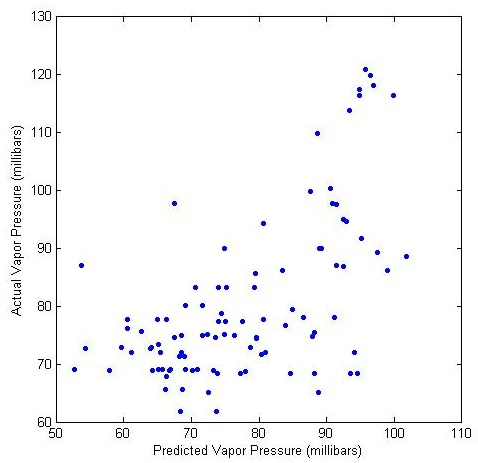
\includegraphics[width=0.45\textwidth]{figures/vaporcorr-nongrad.jpg}
		\label{fig:vaporcorrb}
	}
	\subfigure[]{
		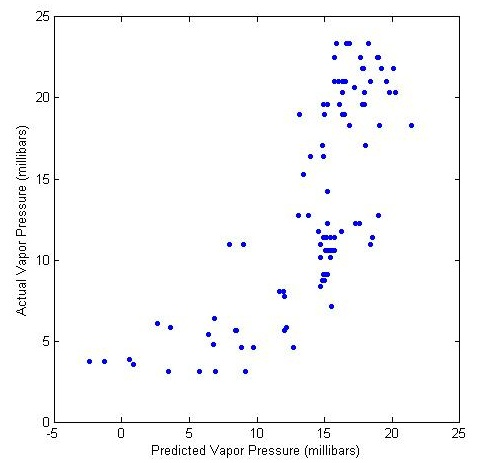
\includegraphics[width=0.45\textwidth]{figures/vaporcorr.jpg}
		\label{fig:vaporcorra}
	}
	\caption[Scatter plots of the predicted vs. actual vapor pressures (in millibars) computed with the regular and gradient images]{Scatter plots of the predicted vs. actual vapor pressures (in millibars) computed with the regular and gradient images, respectively. While the correlation with the regular images (Figure \ref{fig:vaporcorrb}, $r=0.3894$) is poor, there is a noticeable improvement when using the gradient images (Figure \ref{fig:vaporcorra}, $r=0.73684$).}
	\label{fig:vaporcorr}
\end{figure}

Further analysis of our results indicate that vapor pressure is being accurately predicted when the gradient images are used for the training of the predictor. Figure \ref{fig:vaporpred} shows the time series predicted vapor pressure data along with the ground truth values. We see that high vapor pressure measurements clearly indicate more cloudy days, which is exactly what was expected. This example also identifies one failure mode of our algorithm. On March 12, there was such a heavy fog that it obscured the entire scene, making it impossible to accurately predict vapor pressure. This is an unavoidable failure mode as the algorithm depends on the appearance of the image and nothing else to predict the weather. Despite this failure mode, it is clear that the algorithm is able to successfully predict vapor pressure given a reasonable image of the scene.
\begin{figure}
	\centering
	\subfigure[]{
		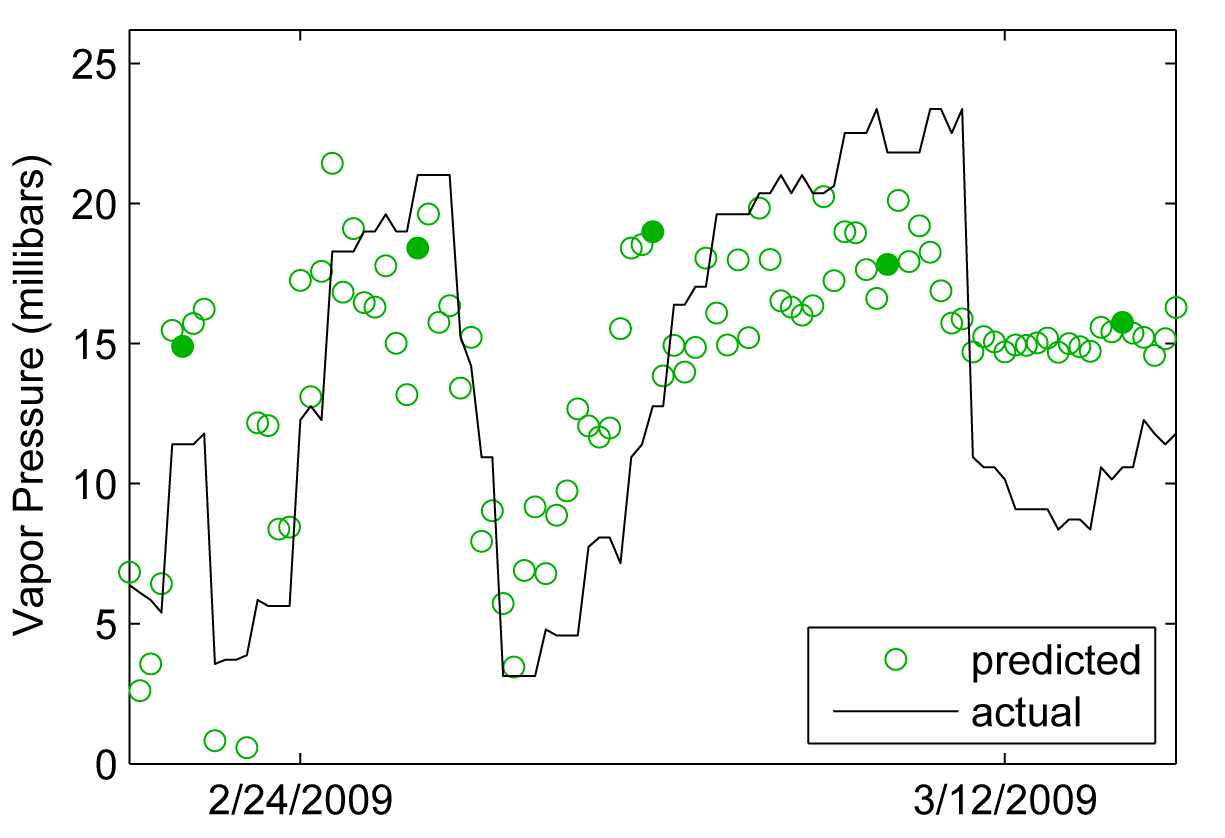
\includegraphics[width=0.60\textwidth]{figures/vaportimeseries-pic.jpg}
		\label{fig:vaportimeseries}
	}
	\subfigure[]{
		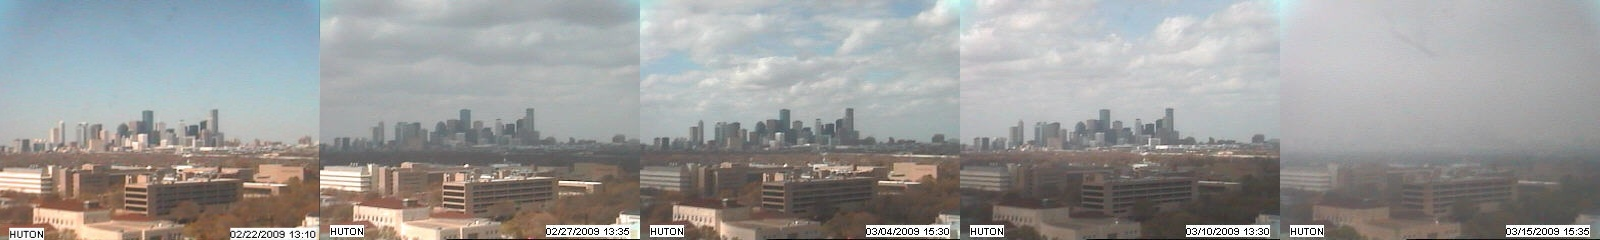
\includegraphics[width=0.90\textwidth]{figures/vaportimeseriesimages.jpg}
		\label{fig:vaportimeseriesimages}
	}
	\caption[Predicted wind speed values and corresponding ground truth values in millibars]{Predicted wind speed values and corresponding ground truth values in millibars shown in Figure \ref{fig:vaportimeseries}. Each image in Figure \ref{fig:vaportimeseriesimages} is associated with one of the filled markers in the plot above. The poor predictions on March 12 are due to heavy fog which obscured the entire scene and left water on the optics.}
	\label{fig:vaporpred}
\end{figure}


\section{Training Size Analysis}
A standard question that must be asked of any machine learning algorithm is: how large of a training dataset is necessary to build a strong model? A strong model is one that can predict our given weather data both accurately \textit{and} precisely. That is, predictions from novel data have small error residuals and are not biased in one direction or the other. The combination of accuracy and precision is a strong argument that the model is truly predicting weather data and not some other signal from the image that is similar to the weather. The goal now is to find the minimum number of data samples needed to build such a model. 

Prior work \cite{barcikowski} using Monte Carlo simulations has suggested that CCA requires the size of the training dataset to be between 40 and 60 times the number of variables being used in correlation analysis. These number were derived from datasets containing between 7 and 41 variables (the sum of number of variables from both sets). The datasets themselves were taken from various actual experiments and were also modified using various regression techniques to make them display certain properties. While this may be true for general cases, we will argue here that far smaller amounts of data are required in our examples due to limited variations and if the samples sufficiently cover the range of possible values.

Recall the wind velocity  and vapor pressure examples used 204 and 198 images to train the CCA projections, respectively. They were tested using 102 and 99 images, respectively. We will now analyze the performance of our algorithms on training sets of various sizes. The images are selected at random from the entire set. The algorithm tests the algorithm 10 times at each training size, varying the images used to train it randomly every time. This helps ensure that we do not get "lucky" with our selections and get an unusually high correlation. Figure \ref{fig:corrcomp} shows how the correlation coefficient $r$ changes as the number of training images changes between 10 and 200 images. Both charts indicate that the average correlation coefficients stop increasing dramatically around 80 images. Additionally, we see that the size of the boxes decreases as the number of images increases. This means that the predictors are more consistent as the number of images increases. This effect is more pronounced in the wind velocity plot (Figure \ref{fig:windcorrcomp}), and is likely due to the increased number of outliers in the vapor pressure plot (Figure \ref{fig:vaporcorrcomp}). Since images are being captured in AMOS every 30 minutes and using 4 hours worth of images for each day, this data indicates that we need just more than 2 weeks of data in order to build a reasonable model of a given weather signal. As wind velocity is a very clear signal, it is not surprising that $r$ converges much quicker in that case.

\begin{figure}
	\centering
	\subfigure[]{
		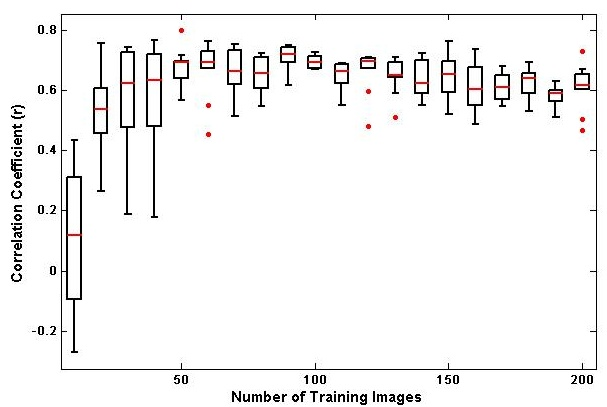
\includegraphics[width=0.70\textwidth]{figures/windspeedtrainsize1.jpg}
		\label{fig:windcorrcomp}
	}
	\subfigure[]{
		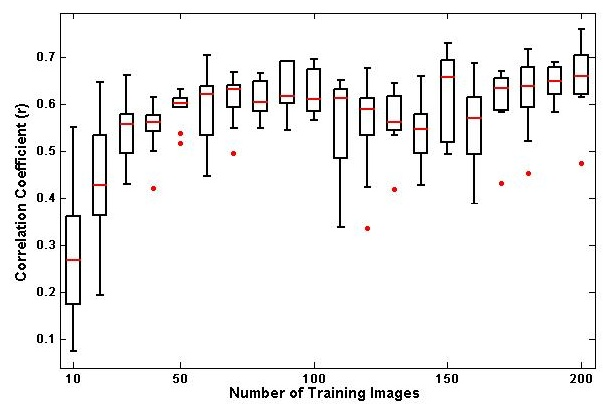
\includegraphics[width=0.70\textwidth]{figures/vaportrainsize1.jpg}
		\label{fig:vaporcorrcomp}
	}
	\caption[Analysis of performance of our algorithms with varying training sizes]{The plots show the correlation coefficient (r) and how it varies with different amount of training data. The values along the line are computed as the average score over 10 different random training sets of the same size. The box and whiskers show the middle two quartiles and outliers, respectively.}
	\label{fig:corrcomp}
\end{figure}

\chapter{Conclusion}
\label{cpt:conclusion}
Images inherently carry with them a vast amount of higher level information. By using regression and correlation techniques, it has been shown in this thesis that we are able to extract very useful information from these images, specifically with regards to weather signals, which vary with time as the images do. By using PCA and CCA, we are able to highlight the important changes occurring in the images and then associate those with weather signals such as wind velocity and vapor pressure. Furthermore, we used the results from a set of tests to determine that just more than 2 weeks of data are required to compute an accurate and precise model. While there is much value in being able to predict weather on an individual camera, such as the ability to fill in holes in reported weather data, the major payoff comes when we are able to predict the weather on many cameras with known locations.

\section{Future Work}
One of the things which makes the AMOS dataset so special and unique is the extremely large number of cameras which is contains. However, only a very few of them are being taken advantage of in this thesis. The algorithm presented in this thesis has been shown to behave well on cameras whose scenes are very different and weather signals that vary as well.

The goal of any future work on this subject should be to further automate the process of finding weather stations close to AMOS cameras, downloading the available weather data, and constantly running, and updating, CCA to predict a variety of weather signals on many cameras. This is very valuable work as it will allow us to analyze local weather patterns across multiple cameras and to infer the weather at other cameras using its location and the locations of other cameras around it. This will allow us to make weather predictions at locations that do not necessarily have a weather station within a reasonable vicinity. 